There exists many places in society where the degree of human occupancy and movement flow is desirable to know as basis for decision making. Such data answers if it is necessary to build more rooms and provides knowledge of actual user or consumer patterns. Example usages are measuring resource usage of public spaces, or which part of a store that attracts most people. It provides vast opportunities in resource management, marketing, sales and scheduling. There exist some plausible solutions to estimating the number of people at a location such as using cell phones or motion detectors, but this project aims at an image based approach with the possible benefits of being both cheaper and more robust.

\subsection{About this document}
This docment, together with the code reference manual (appendix \textbf{??}) constitutes the final documentation of the project and describes the current implementation together with some failed attempts and conclusions drawn from these. Performance results of the current implementation are presented in section \ref{sec:evaluation} of this document.

\subsection{....}

\subsection{Installing the system}
\subsubsection{Hardware}
\subsubsection{Software}
There are two versions of the software, one with a calibration and configuration GUI and one lightweight version without a GUI. In order for the lightweight version to work a configuration file, persumably generated by the GUI version, is required.

\subsection{Calibrating the system}
\subsection{Configuring the system}

\begin{figure}[htb]
	\centering
	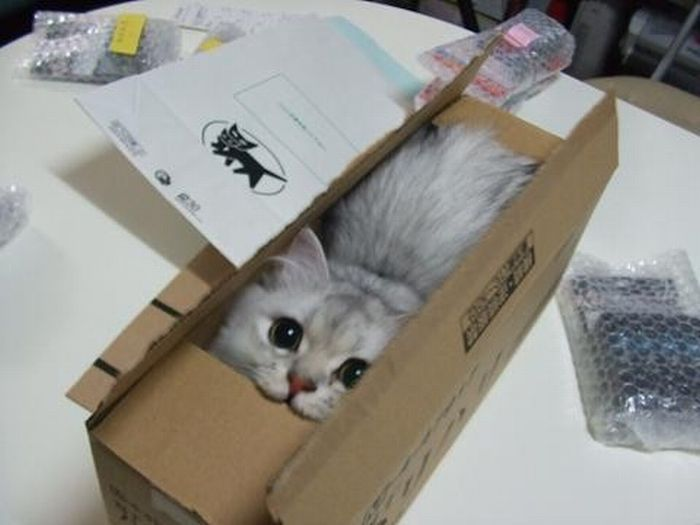
\includegraphics[width=\linewidth]{images/boxcat.jpg}
	\caption[Overview of the entire system]{\textit{System overview.}}
	\label{fig:system_overview}  %Skapar referens till figuren
\end{figure}
